\setchapterpreamble[u]{\margintoc}
\chapter{Deformazione plastica}
\labch{cap7}

Tutti i materiali si possono deformare e, generalmente, la deformazione aumenta in modo proporzionale al carico fino al punto di rottura. Questo tipo di deformazione è del tutto reversibile, essendo in campo elastico.\\
I materiali metallici hanno però in più un comportamento che si differenzia rispetto ad altri tipi di materiali\sidenote{Tipicamente i ceramici presentano solo deformazioni in campo elastico}. Infatti, superato un certo carico, anziché rompersi, cambiano comportamento e la deformazione non è più proporzionale al carico: si ha una deformazione irreversibile e si entra nel campo plastico.

\begin{marginfigure}[-5cm]
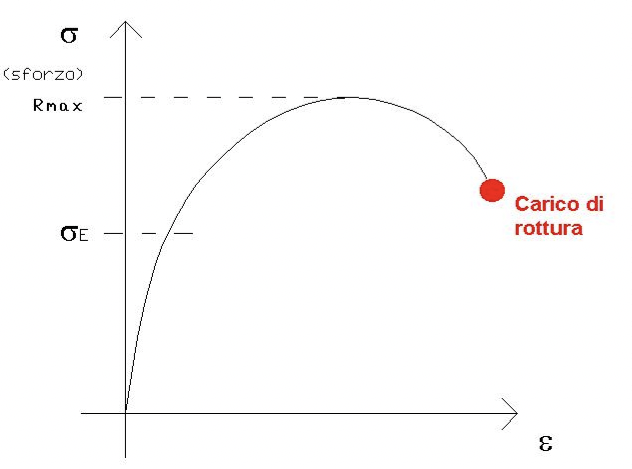
\includegraphics{images/img28.png}
\caption{Diagramma sforzo - deformazione di un materiale duttile}
\labfig{img28}
\end{marginfigure}

\index{deformazione plastica}
Questo comportamento è molto importante sia dal punto di vista produttivo che da quello applicativo: infatti, i materiali metallici possono essere lavorati sia per asportazione di truciolo, sia per deformazione plastica. Esistono tipi di lavorazioni che operano grazie a questa proprietà, come la laminazione, lo stampaggio a caldo e a freddo, la punzonatura, la calandratura, la forgiatura (il materiale viene schiacciato attraverso una pressa o una forgia, solitamente ad alte temperature).\\
La facilità di produzione è certamente molto importante, ma è il comportamento prima della frattura che rende particolarmente prezioni i materiali metallici in campo industriale. Se i materiali fragili si rompono istantaneamente, cioè senza preavviso, e in modo del tutto ingestibile, i materiali metallici prima di rompersi si deformano plasticamente\sidenote{Si definisce \textbf{duttilità} la capacità di un materiale di deformarsi plasticamente prima di giungere a rottura. Un corpo è tanto più duttile tanto maggiore è la deformazione raggiunta prima della frattura.} e quindi, danno il tempo di porre rimedio. \index{duttilità}

Inoltre, l’energia necessaria a portare a rottura un materiale, cioè l’area sottesa alla curva sforzo-deformazione fragile, nel caso di materiale fragile, ad esempio il vetro, è molto piccola, poiché la curva è molto prossima all’asse delle ordinate; un metallo invece prima di rompersi deve assorbire molta più energia\sidenote{Questa proprietà è detta \textbf{tenacità}}.\\ \index{tenacità}
\begin{marginfigure}
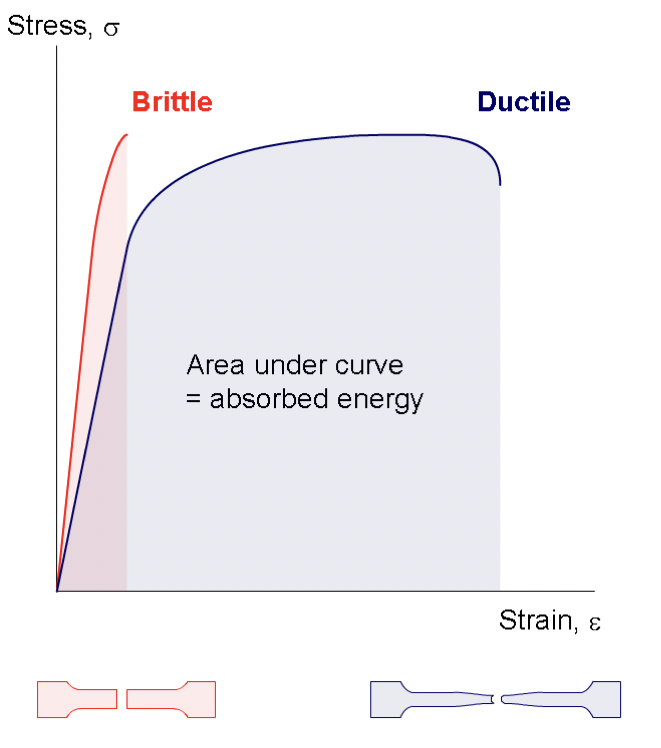
\includegraphics{images/img29.png}
\caption{Tenacità di un materiale fragile e uno duttile a confronto}
\labfig{img29}
\end{marginfigure}

A un certo punto, il materiale in campo plastico comincerà ad assottigliarsi (fenomeno della strizione) fino a rompersi.\\
Ciò vuol dire che i materiale metallici permettono di lavorare in perfetta sicurezza in esercizio: essi hanno carichi di snervamento $\sigma_Y$ e carichi di rottura $\sigma_R$ elevati, cioè sono materiali resistenti, che permettono un alleggerimento della struttura perché non vi è la necessità di sovrapporre molti strati. I materiali metallici hanno elevate caratteristiche meccaniche, che permettono, quindi, di ridurre il peso della struttura.\\
In caso di sollecitazione incidente, l’energia viene utilizzata per la deformazione del materiale e non per la creazione di nuove superfici, cioè non per la rottura. Affinché l’energia assorbita sia elevata, il tratto plastico deve essere molto esteso. Ad esempio, nel campo automobilistico, per la pelle delle automobili si usano materiali in fibra di carbonio, cioè materiali compositi, mentre per l’ossatura è necessario usare materiali metallici\sidenote{Emerge il problema della riciclabilità, cioè di ricaricare interamente il componente, e ciò non è possibile con i materiali polimerici e compositi. I sedili e la loro imbottitura, gli pneumatici non sono riciclabili; i materiali metallici e il vetro, invece, sono gli unici materiali totalmente riciclabili. Ora si sta diffondendo il concetto di re-impiego, cioè si utilizzano i materiali, ad esempio la carrozzeria, per fare altri accessori (declassamento meccanico).}.\\

I materiali metallici sono sicuri, ma anch’essi arrivano alla rottura. Tuttavia, ciò avviene dopo molti “campanelli di allarme”: la deformazione è visibile e per aumentarla, è necessario aumentare il carico. La velocità di deformazione è proporzionale alla velocità di aumento del carico: se il carico aumenta lentamente, la deformazione avverrà lentamente di conseguenza. Ciò permette di operare in sicurezza con i materiali metallici.

\section{Giustificazione delle caratteristiche di deformabilità: i difetti} \index{difetti}

Abbiamo detto che i vetri sono materiali fragili ed assorbono poca energia.
Se i materiali metallici fossero perfetti, non potrebbero avere le applicazioni in cui sono comunemente impiegati e sarebbero, invece, dei “super vetri”, con elevate resistenza e un carico di rottura elevato, ma comunque fragili.\\
In particolare, i difetti che permettono l’elevata deformabilità plastica sono le \textbf{dislocazioni}\index{dislocazioni}, cioè dei difetti di linea. Esse consistono nella mancanza di un semipiano nel reticolo (dislocazione a spigolo).\\
Le dislocazioni sono state prima ipotizzate e poi effettivamente scoperte. Infatti, se si calcola la tensione necessaria a deformare il materiale senza difetti ci si accorge che essa è elevatissima, al contrario di quanto dice l’esperienza.\\
Il movimento delle dislocazioni è favorito dalla presenza di sforzi tangenziali, poiché gli sforzi normali tendono a spezzare il materiale:
\begin{equation*}
    \boldsymbol{\tau = \mathrm{G}\gamma} \quad\text{sforzo tangenziale}
\end{equation*}
dove si sono considerati angoli di deformazione $\gamma$ molto piccoli, tali cioè che $\tan\gamma\simeq\gamma$.\\
Si potrebbe pensare che per determinare una deformazione permanente sia necessario spostare la fila superiore di atomi di una distanza interatomica a. Tuttavia il legame viene spezzato e ricreato con l'atomo successivo già a metà dello spostamento, determinando un angolo $\gamma\simeq1/2$. La $\tau$ teorica in questo caso vale intorno a $10^4\text{MPa}$. I dati sperimentali collocano tuttavia lo sforzo necessario a determinare una deformazione permanete intorno ai 10Mpa.\\
Il ragionamento teorico è difatti valido solo per un materiale perfetto senza difetti: si suppone il sollevamento simultaneo di tutto il piano, la rottura contemporanea di tutti i legami e la ricollocazione del piano stesso in una nuova posizione. In questo caso, si ottengono valori di tensioni molto elevate.

In realtà, con molto meno sforzo, si può creare un’ “onda” che viene fatta scorrere lungo tutto il piano: alla fine del processo, il piano si sarà spostato di una lunghezza pari alla lunghezza d’onda (esempio del tappeto). Tale fenomeno viene identificato nelle dislocazioni.

Nei legami ionici, come ad esempio il gesso (solfato di calcio biidrato $\mathrm{CaSO_4-2H_2O}$) o il sale, che ha una struttura cubica semplice, non c’è movimento dislocativo perché esso porterebbe ioni dello stesso segno a contatto, innescando immediatamente forze repulsive, che causano la rottura del materiale (il materiale si spacca).
Nel legame metallico, invece, i moti dislocativi sono permessi grazie alla presenza della nuvola elettronica: infatti, spostare uno ione non produce alcuna conseguenza.

Si definisce \textbf{vettore di Burgers}\index{vettore di Burger}, \textbf{b}, il vettore che indica lo spostamento delle dislocazioni. Le dislocazioni si muovo lungo direzioni che rendono il vettore di Burgers il più piccolo possibile, poiché l’energia necessaria da fornire affinché una dislocazione si muova è proporzionale a \mathtext{b^2}. Tali piani sono quelli in cui gli atomi sono più vicini, ovvero le distanze interatomiche sono minori: si tratta dei piani a maggiore densità elettronica.\sidenote{Nei reticoli CFC e EC, il vettore di Burgers b è diverso dalla distanza reticolare a e si parla di dislocazioni parziali.}

Nel caso di una cella cubica a facce centrate CFC, i piani con gli atomi più vicini sono quelli diagonali (1 1 1), cioè il piano passante per i tre vertici, nelle tre direzioni <1 $\overline{1}$ 0>. Per ogni cella sono quindi consentiti movimenti in tre direzioni su quattro piani differenti, determinando 12 possibili sistemi di scorrimento.\\
Quindi, il reticolo CFC è quello più sicuro poiché la deformazione avviene in ogni caso. Ne è un esempio l’austenite, che è molto costosa.

Anche nel caso di una cella cubica a corpo centrato CCC, le possibili direzioni per il moto delle dislocazioni sono 12. I sistemi di scorrimento in questo caso però si possono attivare o meno in base alla temperatura. Per temperature maggiori della temperatura ambiente, tutti i sistemi sono attivi e si ha un materia duttile, mentre al di sotto della temperatura ambiente il materiale diventa fragile. Perché la temperatura influenza il moto dislocativo e di conseguenza, la deformazione plastica? All’aumentare delle temperatura aumentano le vacanze che favoriscono il movimento dislocativo.\\
Se vi è un ostacolo, la dislocazione cambia piano di scorrimento: la dislocazione a vite è parallela al vettore di Burgers; quindi può facilmente cambiare piano; la dislocazione a spigolo, invece, è perpendicolare al vettore di Burgers e il piano di scorrimento (all’interno del quale è sempre contenuto il vettore \textbf{b}) è proprio il piano individuato da essi: la dislocazione, quindi, non può cambiare piano.\\
 \textit{Vedi lucidi fenomeni di rafforzamento}.

Esistono dei meccanismi di rafforzamento\index{meccanismi di rafforzamento} per inibire il moto dislocativo:
\begin{enumerate}
    \item  includere nel reticolo di atomi sostituzionali e/o interstiziali: gli atomi interstiziali hanno maggiore potere penetrante e quindi interagiscono sia con le dislocazioni a spigolo sia con quelle a vite, mentre i sostituzionali solo con quelle a spigolo;
    \item incrudimento\index{incrudimento}: le dislocazioni creano altre dislocazioni che interagiscono fra loro, creando degli ingorghi;
    \item  raffinamento dei grani, più il grano è piccolo, più salti vi sono da fare e quindi, deve aumentare il carico. I bordi di grano sono infatti in grado di ostacolare il moto delle dislocazioni. Tale meccanismo aumenta anche la tenacità, bloccando la propagazione delle cricche. Se il grano è grosso, si ha una frattura a nucleazione limitata, dato che una sola cricca può attraversare tutto il grano e rompere il materiale. Se i grani sono piccoli, per portare a rottura il materiale servono più cricche, portando una frattura a propagazione limitata. La rottura dovuta al moto dislocativo avviene a 45°.
\end{enumerate}

\section{Tratto elasto-plastico}

Definiamo il carico nominale: $\sigma_n=\mathrm{P/A_0}$, dove $\mathrm{A_0}$ rappresenta la sezione iniziale.
Definiamo l’allungamento: $\varepsilon=\Delta L/\mathrm{L_0}$\\
Quando si supera la tensione di snervamento $\sigma_Y\simeq\sigma_{02}$ inizia l’incrudimento.
Il tratto seguente viene impropriamente chiamato tratto plastico, quando dovrebbe essere indicato esattamente come tratto elasto-plastico. Quando si scarica il materiale, cioè eliminando il carico $\sigma_{02}$, esso presenta una deformazione plastica residua dello 0,2\%.\\
La retta passante per l’origine e quella passante per la tensione di snervamento in realtà non sono parallele, in quanto il modulo di Young diminuisce all’aumentare della deformazione, poiché si introducono nuove deformazione che diminuiscono la rigidezza del materiale (è come si si introducessero dei buchi nel materiale).

Si ha un effetto di \textbf{springback} o \textbf{ritorno elastico}\index{ritorno elastico}: tutta le deformazione accumulata nel tratto puramente elastico viene recuperata, determinando una deformazione minore rispetto a quella ottenuta con il carico applicato. Questo comportamento è non voluto, perché l’energia elastica viene fornita, quindi rappresenta un costo, e viene restituita in modo talvolta dannoso. Tale effetto deve essere minimizzato, ad esempio, per la produzione degli stampi, dove le tolleranze dimensionali sono minime.

Bisogna, quindi, avere carichi di snervamento bassi, in quanto così si arriva nel tratto plastico con meno sforzo, che si traduce in potenze minori nelle presse e minor ritorno elastico a parità di deformazione.

Negli \textbf{acciai da profondo stampaggio}\index{acciai da profondo stampaggio}, utilizzati per la realizzazione delle carrozzerie, il carico di snervamento è basso.\\
Inoltre, in essi vi sono pochi elementi leganti (tenore di carbonio varia tra lo 0,02\% allo 0,04\%; bassissimi tenori di nichel Ni, silicio Si e magnesio Mg) ed il grano non deve essere fine, ma grosso (comunque non oltre il 20 micron), perché quello fine blocca le dislocazioni.

Il grano deve essere grosso anche per \textbf{leghe per alta temperatura}\index{leghe per alta temperatura}, cioè per le \textbf{superleghe}. Dovendo queste operare a temperature molto elevate possono incorrere nel fenomeno del \textbf{creep}\index{creep}, dove le deformazioni plastiche sono causate non solo dal moto dislocativo, ma anche dallo scorrimento tra grani: quindi avere grani grossi minimizza questo effetto; addirittura si hanno dei precipitati a bordo grano per evitarne lo scorrimento relativo.

Questo comportamento continua fino a quando non si arriva al carico massimo, dove si verifica la una strizione: mentre prima la deformazione era uniforme, con la comparsa delle strizione essa va a localizzarsi solo in una sezione ristretta.\\
Superato il carico massimo, per avere delle deformazioni è necessaria una sollecitazione minore poiché essa agisce su un’area più piccola.\\
In un materiale perfettamente elastico, la componente plastica non va ad aumentare, e sappiamo che si comporta come un materiale fragile, cioè per sforzi maggiori al carico di snervamento, il materiale si rompe.
Quindi la componente plastica è quella che ci permette di sfruttare a pieno le potenzialità del materiale, ed anche il successivo incrudimento.

Nei diagrammi sforzo-deformazione utilizziamo sempre una tensione nominale, calcolata sulla sezione indeformata e si ha un valore nominale della deformazione, proporzionale alla lunghezza di riferimento $\mathrm{L_0}$: $\varepsilon=\Delta L/\mathrm{L_0}=\mathrm{(L-L_0)/L_0}$. Tali valori non rispecchiano l’andamento reale perché l’area varia durante la prova.

Si potrebbe, quindi, usare una tensione reale, riferita alla sezione misurata istante per istante. Dato che in campo plastico vale la legge della conservazione del volume (AL = $\mathrm{A_0L_0}$), si ha che:
\begin{equation*}
    \boldsymbol{\sigma_r}=\mathrm{\frac{P}{A}=\frac{P}{A}\frac{A_0}{A_0}=\sigma_n\frac{A_0}{A}=\boldsymbol{\sigma_n(\varepsilon+1)}}
\end{equation*}
Dove si è usata la conservazione del volume e il fatto che $\mathrm{\varepsilon+1=L/L_0}$.

Un discorso analogo può essere svolto per le deformazioni: nelle prove si misura una lunghezza iniziale \mathtext{L_0}. Quando il materiale comincia a deformarsi si ha una deformazione pari a \mathtext{(L_1-L_0)/L_0}. Nella deformazione successiva si partirà da una lunghezza iniziale $\mathrm{L_1}$ e si avrà \mathtext{(L_2-L_1)/L_1}.
La deformazione reale si può quindi scrivere come:
\begin{equation*}
    \varepsilon_r=\sum_n\frac{L_{n+1}-L_n}{L_n}
\end{equation*}

Passando all’integrale tra \mathtext{L_0} ed L si ottiene 
\begin{equation*}
    \varepsilon_r= \ln(L/L_0)=\ln(\varepsilon+1)
\end{equation*}

Visto che il logaritmo in campo elastico si può confondere con il suo argomento, vale la legge di Hooke \mathtext{\sigma = E\varepsilon}.\\
In campo plastico però la legge non è più lineare, ma vale una relazione del tipo \mathtext{\sigma_r=K\varepsilon_r^n}, dove n è il coefficiente di incrudimento, che determina la pendenza del tratto plastico.\\
\begin{marginfigure}[-4cm]
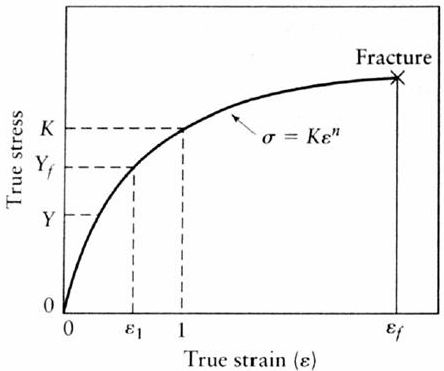
\includegraphics{images/img30.png}
\caption{Diagramma sfrozo - deformazione reali}
\labfig{img30}
\end{marginfigure}
Nel caso reale, vi è una diminuzione del carico perché si continua a considerare la sezione iniziale \mathtext{A_0}, mentre nella realtà non vi è un massima apparente, ma si hanno curve monotone crescenti, in cui non è evidente il carico massimo.\\
Se n=0 avremo un materiale perfettamente plastico (caratterizzato da una curva $\sigma-\varepsilon$ orizzontale), se invece n=1 avremo un materiale perfettamente elastico. Dunque nella realtà 0<n<1.\\
Si cerca di avere un materiale con il coefficiente di incrudimento più alto possibile, perché all’aumentare di n aumenta anche la differenza di carico permessa nel tratto plastico, il che si traduce in una maggiore facilità di lavorazione.

In condizione di carico massimo, si ha:
\begin{align*}
    & (dF)_{max} = 0 \Rightarrow \sigma dA + A d\sigma = 0 \Rightarrow \frac{d\sigma}{\sigma} = -\frac{dA}{A}\\
    & \text{Vol. cost} \Rightarrow ldA + Adl = 0 \Rightarrow \frac{dA}{A} = -\frac{dl}{l}\\
    & \frac{d\sigma}{\sigma} = \frac{dl}{l} = d\varepsilon \Rightarrow \boxed{\frac{d\sigma}{d\varepsilon} = \sigma}
\end{align*}
 la derivata della tensione rispetto alla deformazione è uguale alla tensione stessa e in particolare, introducendo l’espressione di \mathtext{\sigma_r} in condizioni di carico massimo, si ottiene che \mathtext{\varepsilon_{F_{max}}=n}.\\
Infatti, a parità di carico di snervamento, se aumenta n, aumenta anche la deformazione a carico massimo, quindi il materiale è molto più deformabile e stampabile.

Ricapitolando, per avere un \textbf{materiale facilmente stampabile}, bisogna avere basse tensioni di snervamento, alti coefficienti di incrudimento, elevati moduli elastici (per evitare il ritorno elastico) ed elevato coefficiente di anisotropia R\index{coefficiente di anisotropia}.

L’anisotropia è una misura di quanto le proprietà sono le stesse in ogni punto del materiale.
Si definisce coefficiente di anisotropia R la quantità:
\begin{equation*}
    \mathtext{R = (D_{longitudinale} + D_{trasversale} + 2D_{45°}) / 4 = (L + T +2D_{45°}) / 4}
\end{equation*}
D indica la deformazione, L è la deformazione longitudinale e T è la deformazione trasversale.

Un materiale deformato solitamente si allunga nella direzione di applicazione del carico e si assottiglia nelle altre due direzioni. Nel caso di lamiere sottili (1 mm, 0.8 mmm, 0.6 mm) è pericoloso se esse si assottigliano troppo nel senso dello spessore, poiché diminuisce la resistenza della struttura (fenomeno dello \textbf{stone chipping}, ovvero la perforazione di marmitte o pezzi meccanici posti sotto la carrozzeria a causa dei sassi lanciati dagli pneumatici).

E’ preferibile avere R molto elevato, cioè un manufatto che si allunga, ma non si assottiglia.\\
Per sfavorire l’assottigliamento bisogna inibire la crescita dei piani dove si muovono le dislocazioni nel senso dello spessore.

Nella produzione degli acciai, in fase di produzione si ha prima un’ossidazione nel convertitore e poi il calmaggio. Si introduce dell’alluminio Al, che in parte forma dell’ossido portando via dell’ossigeno, ma una percentuale dello 0,04\% rimane nell’acciaio. Tale tenore di alluminio è responsabile dell’anisotropia: infatti, si formano nitruri di alluminio (Al + N), che rimangono in soluzione nell’acciaio, cioè rimangono intrappolati.\\
Dopo il calmaggio, si ha una laminazione a caldo alla temperatura più alta possibile per evitare la precipitazione di tali nitruri. Per arrotolare successivamente la lamiera, bisogna mantenersi a temperature basse, sempre per evitare la precipitazione di tali nitruri.\\
Si può così effettuare la laminazione a freddo, a seguito della quale si ha una ricottura, ad una temperatura di circa 700 - 750 °C, durante la quale deve precipitare il nitruro di alluminio.